\documentclass[10pt,landscape,a4paper]{article}
\usepackage{multicol}
\usepackage[landscape]{geometry}
\usepackage{hyperref}
\usepackage[utf8]{inputenc}
\usepackage{minted}
\usepackage{graphicx}
\usepackage[binary-units]{siunitx}
\usepackage[usenames]{xcolor}
\usepackage{ulem}
\usepackage[english]{babel}
\usepackage{blindtext}
\usepackage{fontspec}
\setmainfont{Arial}
\setlength{\tabcolsep}{0.5em}
\geometry{top=0.5 cm,left=1.5cm,right=1cm,bottom=0.5cm}

% Turn off header and footer
\pagestyle{empty}
 
% Redefine section commands to use less space
\makeatletter
\renewcommand{\section}{\@startsection{section}{1}{0mm}%
                                {-.5ex plus -.5ex minus -.2ex}%
                                {0.5ex plus .2ex}%x
                                {\normalfont\large\bfseries}}
\renewcommand{\subsection}{\@startsection{subsection}{2}{0mm}%
                                {-.5ex plus -.5ex minus -.2ex}%
                                {0.5ex plus .2ex}%
                                {\normalfont\small\bfseries}}
\renewcommand{\subsubsection}{\@startsection{subsubsection}{3}{0mm}%
                                {-.5ex plus -.5ex minus -.2ex}%
                                {0.5ex plus .2ex}%
                                {\normalfont\footnotesize\bfseries}}
\renewcommand{\paragraph}{\@startsection{paragraph}{3}{\z@}%
                                {-.5ex plus -.5ex minus -.2ex}%
                                {-.5em}%
                                {\normalfont\scriptsize\bfseries}}
\makeatother

\setcounter{secnumdepth}{0}

\setlength{\parindent}{0pt}
\setlength{\parskip}{0pt plus 0.5ex}

\usepackage{enumitem}
\setlist{nosep}

%Define Colors
\definecolor{reg1}{HTML}{D6B656}
\definecolor{reg2}{HTML}{6C8EBF}
\definecolor{reg3}{HTML}{82B366}

\definecolor{green}{HTML}{4f9c45}
\definecolor{blue}{HTML}{0000ff}
\definecolor{red}{HTML}{ff0000}

%C-Code inline
\newcommand{\prgc}[1]{\mintinline{C}{#1}}

% -----------------------------------------------------------------------

\begin{document}

\footnotesize
\begin{multicols*}{4}

\setlength{\premulticols}{1pt}
\setlength{\postmulticols}{1pt}
\setlength{\multicolsep}{1pt}
\setlength{\columnsep}{2pt}

\textbf{Zweierkomplement}: invertieren + 1

\subsection{Prozessor-Ablauf}
\textbf{Prozessor...} 1. ...fordert Wert von Adresse an, beim Befehlszeiger. 
2. ...decodiert Instruktion aus Wert.
3. ...wählt den zur Instruktion gehörenden Baustein aus.
\textbf{Aktiver Baustein...} 4. ...decodiert Parameter aus Wert.
5. ...liest aus den Registern.
6. ...führt Berechnung aus.
7. ...schreibt in die Register.
8. \textbf{Prozessor} erhöht Befehlszeiger entsprechend der Länge der Instruktion.

\subsection{Byte-Order}
\textbf{32 Bit 87654321:}

Little Endian: 21 43 65 87\\
Big Endian: 87 65 43 21\\

\textbf{Byte} 1 Byte db 0x35\\
\textbf{Word} 2 Byte, dw 0x2135 $\leftrightarrow$ db 0x35, 0x21\\
\textbf{Doubleword} 4 Byte dd 0x2135 $\leftrightarrow$ db 0x35, 0x21, 0x00, 0x00\\
\textbf{Quadword} 8 Byte dq\\
\textbf{Double Quadword} 16 Byte

\subsection{Register}

instruction pointer: ip in 16-bit, eip in 32-bit, rip in 64-bit

\includegraphics[scale = 0.3]{assembler.png}\\
\begin{tabular}{lllll}
1 & RAX     & \textcolor{reg1}{EAX}     & \textcolor{reg2}{\textit{AX}} & \textcolor{reg3}{AL}\\
2 & RBX     & \textcolor{reg1}{EBX}     & \textcolor{reg2}{\textit{BX}} & \textcolor{reg3}{BL}\\
3 & RCX     & \textcolor{reg1}{ECX}     & \textcolor{reg2}{\textit{CX}} & \textcolor{reg3}{CL}\\
4 & RDX     & \textcolor{reg1}{EDX}     & \textcolor{reg2}{\textit{DX}} & \textcolor{reg3}{DL}\\
5 & RSI     & \textcolor{reg1}{ESI}     & \textcolor{reg2}{SI} & \textcolor{reg3}{SIL}\\
6 & RDI     &  \textcolor{reg1}{EDI}    & \textcolor{reg2}{DI} & \textcolor{reg3}{DIL}\\
7 & RSP     & \textcolor{reg1}{ESP}     & \textcolor{reg2}{SP} & \textcolor{reg3}{SPL}\\
8 & RBP     & \textcolor{reg1}{EBP}     & \textcolor{reg2}{BP} &  \textcolor{reg3}{BPL}\\
9 & R8-R15  & \textcolor{reg1}{R8D-R15D} & \textcolor{reg2}{R8W-R15W} & \textcolor{reg3}{R8L-R15L}
\end{tabular}\\
1. Accumulator, 2. Datenpointer, 3. Counter für Schleifen, Stringoperationen, 4. Pointer für I/O-Operationen,
5. Quelindizes für Stringoperationen, 6. Zielindizes für Stringoperationen, Exitcode, 7. Stackpointer, Adresse des allozierten Stacks,
8. Basepointer, Adresse innerhalb des Stacks, Basis des Rahmens der Funktion , 9. Zusätzliche Register
\subsection{Assembler}
mov Ziel, Quelle\\
global x, y; extern z; w\\
\begin{tabular}{lllll}
0010 & l & .text & 0000 & w\\
0000 &  & *UND* & 0000 & z\\
0018 & g & .text & 0000 & x\\
0020 & g & .text & 0000 & y\\
\end{tabular}\\
1.Spalte (Offset), die letzte den Namen\\
2.Spalte (Symbolattribute: g für global und l für lokal)\\
3.Spalte (Sektion (für unsere Fälle .text))\\
extern deklarierte Label z: *UND*\\
\textbf{Deklaration Label}\\
\begin{tabular}{llll}
O-Datei & Assem. & C & Dek.  C\\
lokal & – & global, inter. Linkage & static\\
global & global & global, exter. Linkage & –\\
– & extern & extern & extern\\
\end{tabular}
extern = diesem oder anderen File deklariert\\
lokal = nicht rausgeben\\
global = anderen o-files zur verfügung stellen
\subsection{Adressierungsmodi}
(Displacement): mov rax, [0x1000]\\
(Base): mov rax, [rcx]\\
(Index * Scale): mov rax, [rbx * 4]\\
\textbf{Label} nicht übersetzt, Offset des nachfolgenden Befehls assoziiert

\subsubsection{Arrays}
\textcolor{red}{Startadresse},
Offset = \textcolor{green}{Index} $ \cdot $ \textcolor{blue}{Variablengrösse in Byte}\\
add rax, [\textcolor{red}{a} + \textcolor{green}{0} *  \textcolor{blue}{8}]

\subsection{Arithmetische und logische Operatoren}
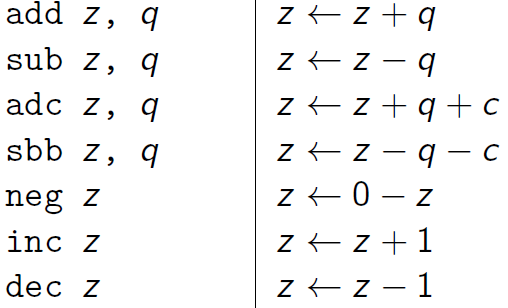
\includegraphics[scale = 0.25]{operatoren.PNG}\\
\begin{tabular}{lll}
Bits & Res. MSBs & Res. LSBs \& 2.Operand\\
64 & RDX & RAX\\
32 & EDX & EAX\\
16 & DX & AX\\
8 & AH & AL\\
\end{tabular}\\
\textbf{mul rbx}, dass RDX:RAX $\leftarrow$ RAX · RBX\\
\textbf{imul} Signed verwendet nur LSB\\
\textbf{div und idiv} wie mul; Quotienten in LSB, Rest in MSB
\begin{multicols}{2}
\subsubsection{Links-Shift}
Multiplikation einer Binärzahl mit $2^{m}$\\
1111 Linksshift um $2^{1}$ = 1111\textcolor{red}{0}  

\subsubsection{Rechts-Shift}
Division einer Binärzahl um $2^{m}$\\
1111 um $2^{1}$  = \textcolor{red}{0}111
\end{multicols}

\subsubsection{Sign-Extension  (Arithmetischer Rechts Shift)}
Statt \textcolor{red}{0} wird links \textcolor{red}{das Vorzeichen} reinkopiert

\subsection{Relative Sprünge}
JMP zahl = RIP$\leftarrow$RIP + zahl\\
JMP label = RIP$\leftarrow$label
\subsection{Flags}
gemeinsames Register RFLAGS\\
\textbf{Carry Flag - CF} Überlauf unsigned\\
\textbf{Overflow Flag - OF} Überlauf signedwerden immer beide bestimmt\\
\textbf{Zero Flag - ZF} Resultat = 0\\
\textbf{Sign Flag - SF} MSB des Resultats\\
\textbf{Parity Flag - PF} niederwertigste Byte = gerade Anzahl 1

\subsubsection{Condition Codes}
\begin{tabular}{lll}
\textcolor{blue}{CC} & Name &  Flags\\
\hline
\textcolor{blue}{A}   & Above             & CF = 0 und ZF = 0\\
\textcolor{blue}{AE}  & Above or Equal    & CF = 0\\
\textcolor{blue}{B}   & Below             & CF = 1\\
\textcolor{blue}{BE}  & Below or Equal    & CF = 1 oder ZF = 1\\
\textcolor{blue}{E}   & Equal             & ZF = 1\\
\textcolor{blue}{G}   & Greater           & ZF = 0 and SF = OF\\
\textcolor{blue}{GE}  & Greater or Equal  & SF = OF\\
\textcolor{blue}{L}   & Less              & SF $\neq$ OF\\
\textcolor{blue}{LE}  & Less or Equal     & ZF = 1 und SF $\neq$ OF\\
\textcolor{blue}{PE}  & Parity Even       & PF = 1\\
\textcolor{blue}{PO}  & Parity Odd        & PF = 0
\end{tabular}

verwirft Ergebnis, setzt Flags:\\
\textbf{cmp}: cmp rax, rbx berechnet RAX – RBX\\
\textbf{test}: test rax, rbx berechnet RAX \& RBX

\subsubsection{Bedingte Anweisungen}
CMOV\textcolor{blue}{cc}: Conditional MOV, J\textcolor{blue}{cc}: Conditional JMP, SET\textcolor{blue}{cc}: Schreibt 1 ins 8-Bit grosse Ziel, wenn \textcolor{blue}{CC} erfüllt, sonst 0 

\subsection{Stack}
\textbf{Calling Convention} Vereinbarung zw. Caller \& Callee. Wird durch Betriebssystem bestimmt:
Argumente, Rückgabewerte, Register bewahren, wer setzt Stackframe?

\textbf{Prolog Funktion:} push rbp; mov rbp, rsp\\
\textbf{Epilog Funktion:} mov rsp, rbp; pop rbp\\
\textbf{call} x legt die nächste Adresse auf den Stack und springt zu x\\
\textbf{ret} nimmt die Rucksprungadresse vom Stack und springt dahin\\
sub rsp , 0x20 ; allocates 0x20 Bytes on stack\\
add rsp , 0x20 ; deallocates 0x20 Bytes on stack
\hline
\subsection{C}
1. Präprozessor\\
2. Compiler\\
3. Assembler .asm $\rightarrow$ Objektdatei/Binärsequenz .o\\
4. Linker mehrere .o-Dateien $\rightarrow$ Executable

\textbf{Objekt-Datei}: Enthält Binärsequenzen\\

\textbf{Executable}: Jedes Symbol erhält einen eigenen, festen Platz im Executable

\subsubsection{Präprozessor}
\textbf{1. Durchlauf}\\ 
Entfernen aller Kommentare, fortgesetzte Zeile $\rightarrow$ in eine Zeile

\textbf{2. Durchlauf, Tokenization}\\ 
\textbf{Bezeichner}: 
\sout{Sonderzeichen}, zusammenfassen: "", escapen

\textbf{3. Durchlauf}\\
Präprozessor-Direktiven (\#) ausführen, Makros durch Expansion ersetzen \\
<file.h> Systemfolder, "file.h" aktuelles Verzeichnis, 

Header 1 / Header 2 $\rightarrow$ Präpozessor $\rightarrow$ Translation Unit $\rightarrow$ Compiler

\subsubsection{Variablen}
globale Variable gleich wie in Assembler, Speicher wird fix reserviert, Grösse durch Typ bestimmt\\
Variable = Label auf Assembler-Ebene

Intialisierung: \prgc{int x = 15;} $\leftrightarrow$ x : dd 15

\subsubsection{Objekt} 
zusammenhängender Speicherbereich, Inhalt kann als Wert interpretiert werden
\textbf{Objektgrösse bestimmen: } \prgc{sizeof(T)}

\subsubsection{Basistypen}
\prgc{char}  8 Bit,
\prgc{short} 16 Bit,
\prgc{int}   16 Bit,
\prgc{long}  32 Bit,
\prgc{long long} 64 Bit\\
default-mässig signed, unsigned muss sonst strikt angegeben werden\\
\textbf{const beezieht sich auf den links ausser wen ganz links dann rechts}\\
\textbf{Mögliche Konvertierungen sizeof(x) vom Stack:} \%i = int, \%X = int(Hexzahl), \%p = void *, \%s = char *
\subsubsection{Arrays}
Bezeichner eines Arrays $\rightarrow$ Pointervariable\\
Mit Elementtyp T ist \prgc{a[index]} äquivalent zu \prgc{a + sizeof(T) * index}
\prgc{f(int x[], int len)} = \prgc{f(int* x, int len)}\\
\prgc{size_t} zum iterieren\\
\prgc{size_t n = sizeof a / sizeof a [0];} 
\prgc{// b == 5 ( elements )}\\
\textbf{String iterieren:} \prgc{while (pc != ’\0’)}
\subsubsection{Structs}
\begin{minted}{C}
struct T
{int x; int y;}; 
struct T t, u;
\end{minted}
belegt gleichen Speicherplatz wie \prgc{int x; int y;}einzeln\\
Zugriff: \prgc{t.x = t.y}\\
\prgc{x} gleiche Adresse wie Struct\\
Member müssen im Speicher nicht dicht liegen (Padding möglich)
\hline
\subsection{Cache}
\textbf{Arbeitsbereich} sind alle Speicherzellen, die in einem Zeitraum verwendet wurden

\subsection{Fully Associative Cache (FAC)}
Eintrag i besteht jeweils aus Adresse ai und Datenbyte di = [ai ]:

Zu jeder Zeile ein Hardware-Baustein, der den Tag t überprüft
Überprüfung wird parallel gemacht\\
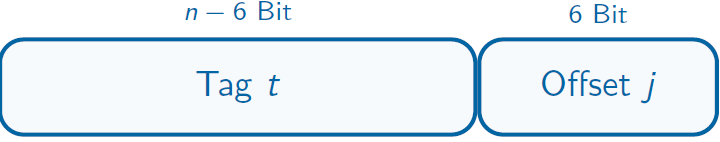
\includegraphics[scale = 0.25]{fac.PNG}

+ Lokalitätsprinzip bestmöglich ausgenutzt\\
- Lookups benötigen viel Hardware und sind teuer

\subsection{Direct-Mapped Cache (DMC)}
Anzahl Einträge/Zeilen = $2^{s}$\\
eine Cachezeile nur an einem einzigen Ort möglich\\
\textcolor{blue}{Index} des Eintrags wird durch die untersten \textcolor{blue}{s} Bit des Tags bestimmt\\
Gespeichert wird nur das reduzierte Tag
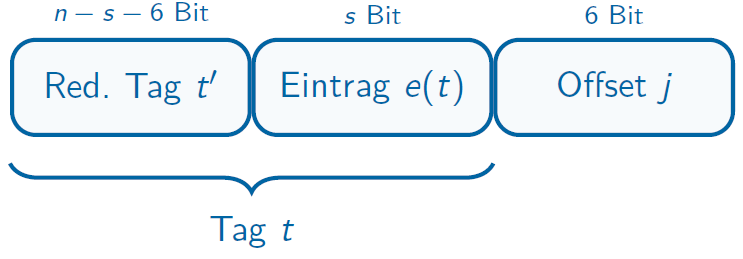
\includegraphics[scale = 0.25]{dmc.PNG}

\subsubsection{Lookup}
ein einziger Vergleichsbaustein\\
Vorgehen: 1. hinteren 6 Byte abschneiden 2. Hintere \textcolor{blue}{s} bits nehmen und an die Index-Stelle gehen 3. Rest der Adresse mit Reduziertem Tag vergleichen. 

+ einfach zu implementieren
+ sehr schneller Lookup
- viele Kollisionen ($1234_h$, $AB34_h$ bei s=8 gleicher Eintrag)

\subsection{Set-Associative Cache (SAC)}
parallele Verwendung von \textcolor{blue}{k} Direct-Mapped Caches\\
Jede Cachezeile kann in \textcolor{blue}{k} Einträgen gespeichert werden\\
Anzahl Set = \textcolor{blue}{k}\\
Jeder DMC = WAY\\
Set-Nummer = Nummer des Eintrags \textcolor{brown}{i}\\
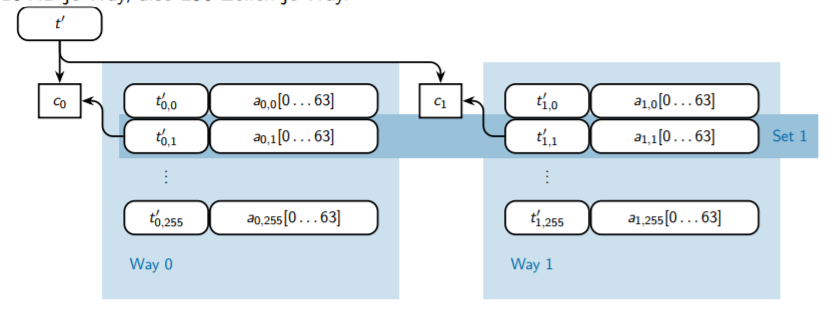
\includegraphics[scale = 0.45]{set-associative.PNG}\\

weniger komplex als FAC,
weiniger Kollisionen als DMC,
Genau so schnell wie FAC und DMC

\hline
\subsection{Random Access Memory (RAM)}
\subsection{Dynamischer Speicher (Heap)}
Nur \underline{explizite} Speicherfreigabe durch OS vorgesehen:\\
\textbf{Reservieren: }\prgc{void * malloc (unsigned int s)}\\
Reserviert Speicherblock der Grösse s\\
gibt Adresse des allozierten Speicherblocks zurück\\
\textbf{freigeben: }\prgc{void free (void* p)}\\

\textbf{Interne Fragmentierung: }grösserer Speicherblock als benötigt
\textbf{Externe Fragmentierung: }Programm reserviert immer wieder Speicher, gibt unregelmässig frei

\subsection{Feste Blockgrösse}
\textbf{Dezentrale Speicherung: }Überläufe
\textbf{Zentrale Speicherung: }Speicherplatz muss extra reserviert werden 
\textbf{Bitlisten: }0 Block ist frei, 1 verwendet
\textbf{Verkettete Listen: }Status(frei?), Start(Adresse erster Block), Size(Anzahl Blöcke), Next(Pointer nächstes Listenelement)\\
Bei Freigabe wird geprüft ob vordere/hintere Teil ebenfalls frei ist und bei Möglichkeit verschmolzen.

\subsubsection{Suchalgorithmen}
\textbf{First Fit:} Wählt erste passende Lücke am Anfang
\textbf{Next Fit:} Wählt erste passende Lücke nach zuletzt reserviertem Bereich
\textbf{Best Fit:} Durchsucht alle Lücken und wählt die kleinste passende aus
\textbf{Worst Fit:} Durchsucht alle Lücken und wählt die grösste aus

\subsubsection{Grössenklassen}
Bereiche nur in bestimmten Grössen,
freie Bereiche in Liste, \textbf{Quickfit: }wählt kleinstpassenden aus Liste
+Schnelle Reservation, -Nachbarn sind nicht leicht zu finden

\subsubsection{Buddy-System}
Wenn 2 Bereiche gleiche bits bis auf einen $\rightarrow$ Buddies
\subsubsection{Objekt-Pools}
Speicherbereich fester Grösse(Page) in kleinere Bereiche, keine Rekombi bei Rückgabe,
Mehr Objekte?$\rightarrow$neue Page, Freie Objekte in Freiliste\\

\hline
\subsection{Programmstart/-ende}
Seperates Register für Syscalls: IA32\_LSTAR
Intel Prozessoren haben Privilege-Levels: 0 = OS, 3 = Programme\\
mov rax, [Funktionscode];
mov rdi, [weitere Argumente];
syscall;
\subsection{Virtueller Speicher (Hardware)}
MMU (Memory Management Unit) übersetzt Virtuelle in reale Adresse\\
Pro Prozess eine Page-Table\\
OS stellt Übersetzungs-Mapping bereit. Prozesse bekommen keine realen Adressen mit\\
Bei falschem Zugriff $\rightarrow$ Fault-Interrupt $\rightarrow$ OS übernimmt\\
OS lagert nicht benötigtes aus, OS lädt fehlende inhalte vom Sekundärspeicher
Pages normalerwiese 4KB gross\\
Hauptspeicher besteht aus Pageframes\\
Wenn Pages (4kb/12bit) Hauptspeicher-Adresse = 0x AB 78 90 00 $\rightarrow$ Page Frame Number = 0xAB789\\ 
Page = Daten
\subsubsection{Single-Level Page-Table}
ein Eintrag pro Page
+ Lookup sehr schnell $\rightarrow$ Index = PageNumber

\subsubsection{Two-Level Page-Table}
Page Number wird aufgeteilt: Directory Index (nur eine!), Page Table Index (zweidimensionales Array)
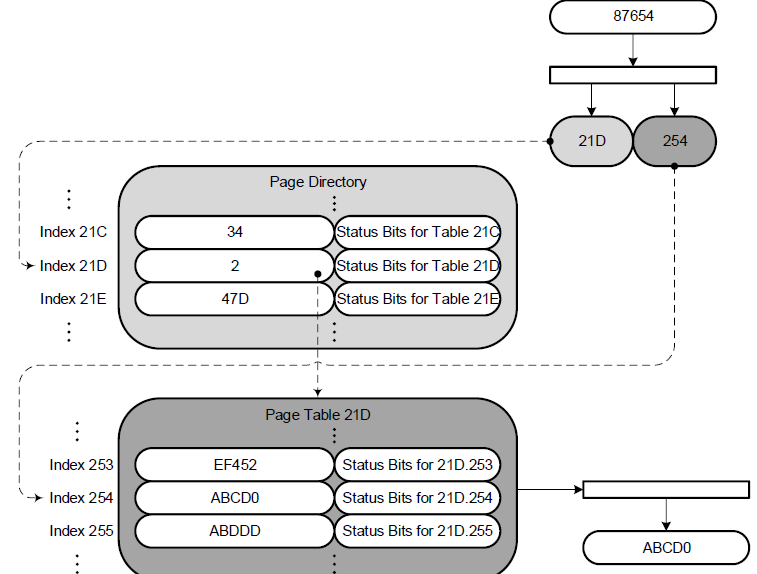
\includegraphics[scale = 0.3]{Two-level-page.PNG}\\
\subsubsection{Multi-Level Page-Table}
Page Directory Pointer Table, Page Directory, Page Table
\textbf{Translation Lookaside Buffer: }Cache für häufig benu. Mappings

\subsection{Virtueller Speicher (Software)}
Unterstes Bit = P-bit (Present) (1 = im Hauptspeicher)\\
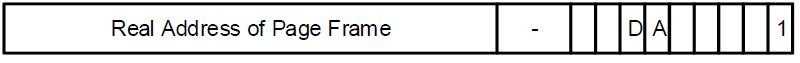
\includegraphics[scale = 0.3]{page.PNG}\\
MMU setzt A-Bit/«Accessed» bei jedem Zugriff auf Page,
D-Bit/«Dirty» bei jedem Schreibzugriff auf Page$\rightarrow$zurückschreiben in HDD\\
OS kann beide bits löschen\\
Wenn  P-bit = 0 $\rightarrow$ Der Platz davor wird dafür verwendet, wo die Page im Sekundärspeicher liegt\\
Wenn Page nicht alloziert ist $\rightarrow$ Schutzverletzung\\
Nachdem Page geladen wurde wiederholt MMU den Zugriff

\subsection{Dreschen/Häufiges Pagen}
Hauptspeicher viel zu klein/zu viele Prozesse$\rightarrow$mehr Hauptspeicher, 
Beschränkung Anz. Prozesse, 
Verminderung Paging-Strategien

\subsection{Ladestrategien RAM$\leftarrow$HDD}
Beeinflusst Häufigkeit von Pagefaults\\
\textbf{Demand Paging: }Laden auf Anfrage, +min. Aufwand, -lange Wartezeiten
\textbf{Prepaging: } Seiten frühzeitig geladen
\textbf{Demand Paging mit Prepaging: }wie Demand + benachbarte Pages(Lokalitätpr.),
+weniger Page-Faults, +Blocktransfer, -Manchmal unnötiges Laden

\subsection{Entladestrategien RAM$\rightarrow$HDD}
Beeinflusst Zeit bei Pagefaults\\
\textbf{Demand Cleaning: }nur geschrieben wenn nötig, +min. Aufwand, -erhöhte Wartezeit
\textbf{Precleaning: }Vorausschauendes Schreiben, +reduzierte Wartezeit, -wenn Pages nach Schreibvorgang nochmals geändert
\textbf{Page Buffering: } 2 Listen: \textbf{U}nmodified Pages (zuerst ersetzt), \textbf{M}odified Pages\\
OS schreibt von M in Secondärspeicher/ OS schiebt von U zu M wenn Dirtybit gesetzt.  +/-Precleaning, +schnelle Auswahl beim Ersetzen

\subsection{Verdrängungsstrategien}
\textbf{Beladys Anomalie:} Grösserer Hauptspeicher kann zu mehr Page Faults führen
\textbf{Optimal: }spätesten in Zukunft gebraucht
\textbf{FIFO: }Problem: alte, häufig benutzte Pages werden gelöscht und gleich wieder geladen
\textbf{Second Chance: }FIFO + prüft Referenced-Bit, 0=weg, 1=hinten + 0
\textbf{Clock: }
Effiziente Impl. Second Chance: Linked List im Kreis. Pointer wird nur verschoben
\textbf{Least Recently Used: }ersetzt längste unbenutzte Page, notiert Zeitpunkt in Page-Table, + sehr nahe am Optimum
- grosser Aufwand in HW, Page-Einträge grösser
\textbf{Working Set: } Pro Page-Interrupt\\ R==1: t = now setzen,R==0: now - t$<$Working Set T$\rightarrow$JA: Page behalten / NEIN: Page entfernen
\hline

\subsection{In-/Output}
\textbf{Memmory-mapped I/O: }pro Gerät 1 Adressbereich, -Adressbereich kann nicht für Speicher benutzt werden, +Einfachheit
\textbf{Port-mapped I/O: }separater Bus, zwei Adressräume (Speicher und Geräte), Pro Adressraum eigene Instruktionen, -Komplexität
\textbf{Port-mapped I/O via Memorybus: }gemeinsamer Bus, zusätzliche Bitleitung für Speicher|I/O, Adressraum wird um 1 Bit erweitert, +Ganzer Adressraum, +einfaches Design
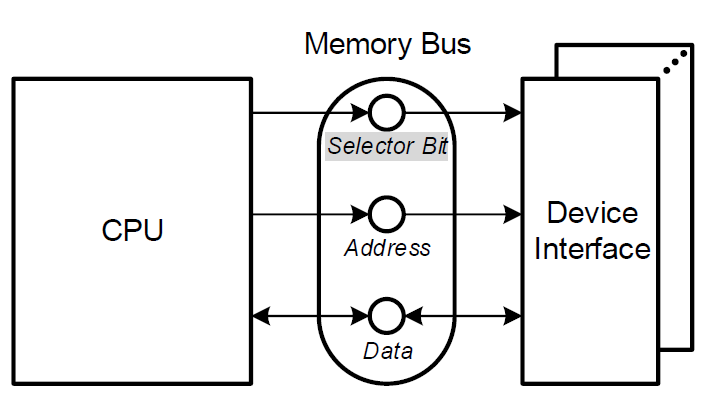
\includegraphics[scale = 0.2]{memorybus.PNG}
\subsubsection{Kommunikationsmechanismen}
\textbf{Programmgesteuert/Polling} Programm fragt die ganze Zeit ab, +Keine Verzögerung, -Legt CPU lahm
\textbf{Polling ohne Busy-wait} Programm pollt in Abständen, -erfordert zeitliche analyse, +CPU kann etwas anderes tun
\textbf{Interruptgesteuert}: Device meldet sich wenn Ready, Prozessor hat Interrupt Pin + \textcolor{red}{Interrupt Number}. Prozessor hat Interrupt Vector Table(Tabelle mit Funktionen), welche der Prozessor anhand der \textcolor{red}{Interrupt Number} aufruft
Nach Instruktion prüfen ob interupt Pin gesetzt ist. Ja $\rightarrow$ unterrbricht Ausführung \& sichert alles
\subsection{Treiber}
\textbf{ohne Treiber} $\rightarrow$ -Sicherheit, -Stabilität, -Komplexität, -Multiprogrammierung
\textbf{Mit Treiber} Benutzerprogramme können nur über OS-API auf Hardware zugreifen\\
Treiber = Komponente zur Kommunikation mit HW / Separat ins OS integrierbar / können aufeinander aufbauen
\hline
\subsection{Varia}
Nibble = 4 Bit, Oktett = 8 Bit, Byte = Oktett
\textbf{unsigned/ohne Vorzeichen}: $0...2^{n}-1$\\
\textbf{Disjunktion:} $\vee$, \textbf{Konjunktion:} $\wedge$
\begin{multicols}{2}
2$^{30}$ G Giga\\
2$^{40}$ T Tera\\
2$^{50}$ P Peta\\
2$^{60}$ E Exa\\
\end{multicols}
\end{multicols*}
\end{document}